\section{Trigger}

With a $pp$ interaction rate of $40\mhz$ there is clearly too much information associated with an event
to write them all to disk.
Instead a multistage trigger is employed.
The first level trigger, \lone, is embedded in the hardware of \lhcb and is fully synchronous with
the bunch crossing rate.
It uses momentum and energy information to select events.
Its output rate is $1\mhz$.
Two software triggers are fast enough to perform tracking algorithms and use information from
multiple subdetectors to reduce the events written to disk to $5\khz$.
The flow of data through the trigger is shown in Fig.~\ref{fig:lhcb:trigger}.

\begin{figure}
  \begin{center}
    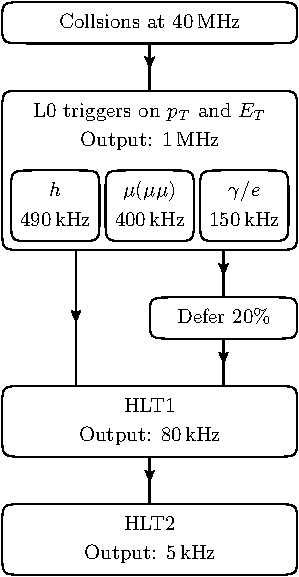
\includegraphics[scale=1]{trigger}
  \end{center}
  \caption[Trigger sequence]
  {\small
    The flow of the \lhcb trigger system in 2012.
  }
  \label{fig:lhcb:trigger}
\end{figure}

There are five \lone trigger lines; one each for photons, electrons, hadrons, muons and dimuons.
The decisions of the former three are based on calorimeter information while th others use muon
system information.
A cluster in the \ecal and \hcal is defined as two-by-two calorimeter cells.
For each cluster the transverse energy, $E_T$, is calculated:
\begin{equation}
  E_T = \sum_{i=1}^4E_i\sin\theta_i,
\end{equation}
where $E_i$ is the energy in cluster $i$ and $\theta_i$ is the angle between the average
interaction point and the cell's centre.
These clusters are then categorized as follows.
A hadron candidate is the largest $E_T$ cluster in the \hcal summed with the $E_T$ of the \ecal
cluster in front, if there is one.
A candidate photon (electron) is the largest $E_T$ deposit with hits in the \presh cells in front and
no hits (at least one hits) in the nearest \spd cells.
The $E_T$ of each candidate is compared to thresholds, and the event is retained if one or more is
exceeded.

First level trigger lines associated with muons base their acceptance on measurements of \pt.
Each quadrant of the muon system is read out independently, so muons which cross boundaries cannot
be triggered.
The muon candidates with the highest and second highest \pt are selected from each quadrant by
searching for straight lines through M1-5 in the $z-y$ plane, and in the $z-x$ plane if
$p_T>0.5\gev$.
The M1 station is used to increase the \pt resolution of tracks, this enables (without the
tracking information) a resolution of about $25\,\%$ of fully reconstructed tracks.
Events are accepted based on candidates from all quadrants with values of $p_T^\mathrm{max}$ and
$p_T^\mathrm{max}\times p_T^\mathrm{2^{nd} max}$ greater than thresholds for the muon and dimuon
lines respectively.
Thresholds for \lone trigger lines used in this thesis are given in \Tab{tab:lhcb:trigger}.

\begin{table}
  \caption{\small
    Thresholds in 2011 and 2012 for \lone trigger lines~\cite{Albrecht:2013fba} used in this thesis.
  }
  \label{tab:lhcb:trigger}
  \begin{center}
    \begin{tabular}{ccc}\toprule
      &2011&2012\\\midrule
      {\tt L0Muon} & $1.48\gev$ & $1.76\gev$ \\
      {\tt L0Dimuon} & $(1.296\gev)^2$ & $(1.6\gev)^2$ \\
      {\tt L0Hadron} & $3.5\gev$ & $3.7\gev$ \\
      \bottomrule
    \end{tabular}
  \end{center}
\end{table}

Around $80\%$ of the events accepted at \lone are processed by the software triggers immediately.
The rest are stored temporarily on hard disks to be processed while the \lhc is not colliding protons.
This is known as deferred triggering.

The first software trigger, \hltone, performs the full three dimensional \velo track fitting
algorithms (but with fewer passes than the offline version).
Candidate \velo tracks for triggers which do not require muons are selected based upon the quality of the
\velo track and the smallest IP with respect to any of the identified primary vertices.
Primary vertices are defined to be points within $300\mum$ of the mean
interaction point in the $x-y$ plane, $\mathrm{PV}^\mathrm{mean}_{xy}$, from which at least five
tracks originate.
The position of $\mathrm{PV}^\mathrm{mean}_{xy}$ is measured at the start of each \lhc machine
fill.
For trigger lines requiring muons, each \velo track is extrapolated to a window in the M3
station.
The size of this window is narrow in the non-bending direction but wide enough to accommodate a $6\gev$
muon in $x$.
If there is a deposit in this window then the \velo track, is extrapolated to the cluster and if
there are hits consistent with this track in any of the muon stations M2, M4 or M5 the track is
tagged as belonging to a muon.
The \velo tracks that are selected by IP or the muon system are extrapolated (or interpolated) into
the \intr and \ot.
This is known as forward tracking, and provides momentum measurements for all these tracks.

More info needed on specific lines?

The second software trigger, \hlttwo, performs forward tracking on all \velo tracks with
$p>5\gev$ and $p_T>0.5\gev$ in 2011; which was reduced to $p_T>0.3\gev$ in 2012 thanks to deferred
triggering.
These charged tracks are then used to identify decaying $B$ mesons using their topology.
Vertices formed of two, three and four reconstructed tracks displaced from PVs are triggered based
on the response of a Bonsai Boosted Decision Tree (BBDT)~\ref{Gligorov:2012qt} whose inputs are
properties of the tracks and vertex.
A BBDT is a Boosted Decision Tree (to be described in an Appendix) where input variables are
discretized allowing a simple, fast look-up table to be used to calculate the trigger
output~\cite{Gligorov:2012qt}.

%Trigger 2011 \cite{LHCb-DP-2012-004}
%Trigger 2012 \cite{Albrecht:2013fba}







\subsection{Lines}
BBDT lines: identify seconday vertices consistent with decay of a B hadron
BBDT-MU lines: identify seconday vertices consistent with decay of a B hadron with nuons in the
final state.


